% !TeX program = lualatex
% ================================================================
% Polish Parallel Text Version of CirclesAreaIdeasStarters
%
% Generated by the server using the following settings:
%
%   language            Polish (pol)
%   text direction      left to right
%   font                Noto Serif
%   fallback font       Noto Serif
%   built from          latex/starters/targeted/KS3/circles/circlesAreaIdeasStarters.tex
%   vocabulary key      latex/starters/targeted/KS3/circles/circlesAreaIdeasStarters/L2/pol/circlesAreaIdeasStarters_polishKey.tex
%   tier 3 vocabulary   green   RGB 0 128 0
%   English text        black   RGB 0 0 0
%   Polish text         purple  RGB 112 48 160
%   layout macros       version 2
%
% Please don't edit any information in this comment block - the server
% compares it against the current settings and rebuilds this file when
% they differ, so changes here would be overwritten. However, feel free
% to make updates to the LaTeX below if you want to edit it.
% ================================================================

\documentclass{beamer}
\usepackage{tikz}
\usetikzlibrary{calc,arrows.meta,patterns}
\usepackage{multicol}
\usepackage{amsmath}
\usetikzlibrary{overlay-beamer-styles}
% Characters this language's font has not got are borrowed from another,
% rather than being silently dropped - see docs/translated-sheet-latex.md
\directlua{%
  if luaotfload and luaotfload.add_fallback then
    luaotfload.add_fallback("eallatinfallback",
      { "Noto Serif:mode=harf;" })
  else
    tex.error("this luaotfload is too old to register a fallback font")
  end
}
\usepackage[english]{babel}
\babelprovide[import]{polish}
\babelfont[polish]{rm}[Renderer=Harfbuzz, BoldFont={Noto Serif}, ItalicFont={Noto Serif}, BoldItalicFont={Noto Serif}, RawFeature={fallback=eallatinfallback}]{Noto Serif}
\babelfont[polish]{sf}[Renderer=Harfbuzz, BoldFont={Noto Serif}, ItalicFont={Noto Serif}, BoldItalicFont={Noto Serif}, RawFeature={fallback=eallatinfallback}]{Noto Serif}
\newcommand{\ealtext}[1]{\foreignlanguage{polish}{#1}}
\newcommand{\ealtextblock}[1]{{\raggedright\foreignlanguage{polish}{#1}\par}}
% ================================================================
% EAL layout helpers
% ================================================================
\usepackage{xcolor}

\definecolor{ealkeycolour}{RGB}{0,128,0}
\definecolor{ealenglish}{RGB}{0,0,0}
\definecolor{ealtwocolour}{RGB}{112,48,160}

\newsavebox{\ealboxen}
\newsavebox{\ealboxtr}
\newlength{\ealglosswd}
\newlength{\ealglossraise}
\setlength{\ealglossraise}{1.15em}

% a tier 3 word, in English and in translation alike
\newcommand{\ealkey}[1]{\textcolor{ealkeycolour}{#1}}
\newcommand{\ealkeytr}[1]{\textcolor{ealkeycolour}{\ealtext{#1}}}

% One translated word above one English word. Built from kernel
% primitives, never a tabular, which would break wherever the sheet
% loads array, booktabs or tabularx. The box is as wide as the wider of
% the two, so a long translation pushes its neighbours aside instead of
% overlapping them, and it claims its full height so a table row or a
% TikZ node makes room for it.
\newcommand{\ealgloss}[2]{%
  \sbox{\ealboxen}{\ealkey{#1}}%
  \sbox{\ealboxtr}{\small\textcolor{ealtwocolour}{\ealtext{#2}}}%
  \setlength{\ealglosswd}{\wd\ealboxen}%
  \ifdim\wd\ealboxtr>\ealglosswd\setlength{\ealglosswd}{\wd\ealboxtr}\fi
  \leavevmode
  \makebox[\ealglosswd][c]{%
    \makebox[0pt][c]{\usebox{\ealboxen}}%
    \makebox[0pt][c]{\raisebox{\ealglossraise}{\usebox{\ealboxtr}}}%
  }%
}

% opens up line spacing around a block of glosses, so the raised
% translations sit clear of the line above
\newenvironment{ealglossed}{\par\linespread{2.1}\selectfont\ignorespaces}{\par}

% a whole translated sentence above its English counterpart. block level,
% so it does not belong inside a tabular cell
\newcommand{\ealpara}[2]{%
  \par\addvspace{0.5\baselineskip}%
  {\color{ealtwocolour}\ealtextblock{#1}}%
  \penalty200
  {\color{ealenglish}#2\par}%
  \addvspace{0.5\baselineskip}%
}

\begin{document}

\frame{\titlepage}

%------------------------------------------------
% SLIDE 1: Retrieval + Squaring as a New Skill
%------------------------------------------------
\begin{frame}{Starter}

\vspace{-2em}

\ealpara{Rozgrzewka}{Starter}

\begin{columns}

\column{0.35\textwidth}
\begin{center}
\begin{tikzpicture}[scale=0.85]
  % Grid of squares to illustrate squaring / area idea
  \draw[gray!40, thin] (0,0) grid (3,3);
  \draw[thick, blue] (0,0) rectangle (3,3);
  \draw[blue, thick, <->] (0,-0.35) -- (3,-0.35);
  \node[blue] at (1.5,-0.65) {$3$ cm};
  \draw[blue, thick, <->] (-0.35,0) -- (-0.35,3);
  \node[blue, rotate=90] at (-0.7,1.5) {$3$ cm};
  \node at (1.5,1.5) {\small $9$ cm$^2$};

  % Small circle below for context
  \draw[thick] (1.5,-2.5) circle (1.5cm);
  \fill (1.5,-2.5) circle (0.04);
  \draw[red, thick] (1.5,-2.5) -- ++(0:1.5);
  \node[red, below] at (2,-2.6) {\small $1.5cm$};

% --- Q9 answer: the r = 1.5 cm circle drawn inside the 3 cm square ---
\draw[ans] (1.5,1.5) circle (1.5cm);
\draw[ans] (1.5,1.5) -- ++(-55:1.5);
\node[anslab, left] at (2.02,0.76) {$1.5$ cm};
\end{tikzpicture}
\end{center}

\column{0.65\textwidth}
\small
\begin{enumerate}
  \begin{multicols}{2}
    \item $4 \times 4 = \ashowq{16}$
    \item $7 \times 7 = \ashowq{49}$
  \end{multicols}
  \begin{multicols}{2}
    \item $10^2 = \ashowq{100}$
    \item $3^2 = \ashowq{9}$
  \end{multicols}
  \item \ealpara{$2 \times 6$ i $6^2$ --- czy to to samo? \ashow{Nie: $12\neq 36$.}}{$2 \times 6$ and $6^2$ --- are these the same? \ashow{No: $12\neq 36$.}}
  \begin{multicols}{2}
  \item $3.14 \times 9=\ablank{28.26}$
  \item $3.14 \times 25=\ablank{78.5}$
  \end{multicols}
\end{enumerate}
\vspace{-1em}
\begin{enumerate}
  \setcounter{enumi}{6}
  \item \ealpara{\ealkeytr{Koło} ma \textbf{\ealkeytr{średnicę}} $14$ cm. Znajdź: (a) \ealkeytr{promień} \ablank{7\,\text{cm}} \newline{} (b) \ealkeytr{obwód} \ablank{43.96\,\text{cm}}. ($\pi \approx 3.14$)}{A \ealkey{circle} has \textbf{\ealkey{diameter}} $14$ cm. Find: (a) the \ealkey{radius} \ablank{7\,\text{cm}} \newline{} (b) the \ealkey{circumference} \ablank{43.96\,\text{cm}}. ($\pi \approx 3.14$)}
  \item \ealpara{\ealkeytr{Koło} ma \textbf{\ealkeytr{promień}} $5$ cm. Jaki jest \ealkeytr{obwód}? \ablank{31.4\,\text{cm}}}{A \ealkey{circle} has \textbf{\ealkey{radius}} $5$ cm. What is the \ealkey{circumference}? \ablank{31.4\,\text{cm}}}
  \item \ealpara{\ealkeytr{Kwadrat} ma bok $3$ cm i \ealkeytr{pole} $9$ cm$^2$. \ealkeytr{Koło} ma \ealkeytr{promień} $1.5$ cm. Czy \ealkeytr{pole} \ealkeytr{koła} jest większe czy mniejsze niż $9$ cm$^2$? \ashow{Mniejsze: $\pi(1.5)^2 \approx 7.07$ cm$^2$.}}{The \ealkey{square} has side $3$ cm and \ealkey{area} $9$ cm$^2$. A \ealkey{circle} has \ealkey{radius} $1.5$ cm. Is the \ealkey{circle}'s \ealkey{area} more or less than $9$ cm$^2$? \ashow{Less: $\pi(1.5)^2 \approx 7.07$ cm$^2$.}}
\end{enumerate}

\end{columns}
\end{frame}

%------------------------------------------------
% SLIDE 2: Retrieval + Radius vs Diameter + Squaring in Context
%------------------------------------------------
\begin{frame}{Starter}

\ealpara{Rozgrzewka}{Starter}

\begin{columns}

\column{0.35\textwidth}
\begin{center}
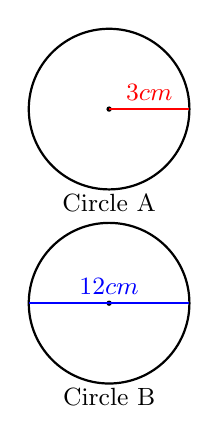
\begin{tikzpicture}[scale=0.85]

  % Circle A — radius labelled
  \draw[thick] (0,2.5) circle (1.2cm);
  \fill (0,2.5) circle (0.04);
  \draw[red, thick] (0,2.5) -- ++(0:1.2);
  \node[red] at (0.6, 2.75) {\small $3cm$};
  \node at (0, 1.1) {\small Circle A};

  % Circle B — diameter labelled
  \draw[thick] (0,-0.4) circle (1.2cm);
  \fill (0,-0.4) circle (0.04);
  \draw[blue, thick] (-1.2,-0.4) -- (1.2,-0.4);
  \node[blue] at (0,-0.15) {\small $12cm$};
  \node at (0,-1.8) {\small Circle B};

\end{tikzpicture}
\end{center}

\column{0.65\textwidth}
\small
\begin{enumerate}
  \begin{multicols}{2}
    \item \ealpara{Podziel na pół $12$ cm \ablank{6\,\text{cm}}}{Halve $12$ cm \ablank{6\,\text{cm}}}
    \item \ealpara{Podziel na pół $9.4$ cm \ablank{4.7\,\text{cm}}}{Halve $9.4$ cm \ablank{4.7\,\text{cm}}}
  \end{multicols}
  \begin{multicols}{2}
    \item $6^2 = \ashowq{36}$
    \item $1.5^2 = \ashowq{2.25}$
  \item $3 \times 4^2=\ablank{48}$
  \item \ealpara{Prawda czy fałsz? $\pi \times (2r) = 2 \times \pi \times r$ \ashow{Prawda}}{True or false? $\pi \times (2r) = 2 \times \pi \times r$ \ashow{True}}
  \end{multicols}
\end{enumerate}
\vspace{-2em}
\begin{enumerate}
  \setcounter{enumi}{6}
  \item \ealpara{Rozważ \ealkeytr{koło} A \newline{} (a) Jaki jest \ealkeytr{obwód}? \ablank{18.84\,\text{cm}} \newline{} (b) Jakie jest \ealkeytr{pole}? \ablank{$28.26\,\text{cm}^2$}}{Consider \ealkey{circle} A \newline{} (a) What is the \ealkey{circumference}? \ablank{18.84\,\text{cm}} \newline{} (b) What is the \ealkey{area}? \ablank{$28.26\,\text{cm}^2$}}
  \item \ealpara{Rozważ \ealkeytr{koło} B \newline{} (a) Jaki jest \ealkeytr{obwód}? \ablank{37.68\,\text{cm}} \newline{} (b) Jakie jest \ealkeytr{pole}? \ablank{$113.04\,\text{cm}^2$}}{Consider \ealkey{circle} B \newline{} (a) What is the \ealkey{circumference}? \ablank{37.68\,\text{cm}} \newline{} (b) What is the \ealkey{area}? \ablank{$113.04\,\text{cm}^2$}}
  \item \ealpara{Czy \ealkeytr{stosunek} \ealkeytr{obwodów} \ealkeytr{kół} A i B jest taki sam jak \ealkeytr{stosunek} \ealkeytr{pól}? \ashow{Nie: $1:2$ wobec $1:4$.}}{Is the \ealkey{ratio} of the \ealkey{circumferences} of \ealkey{circles} A and B the same as the \ealkey{ratio} of the \ealkey{areas}? \ashow{No: $1:2$ vs $1:4$.}}
\end{enumerate}

\end{columns}
\end{frame}

%------------------------------------------------
% SLIDE 3: Retrieval + Area Intuition + First Explicit Area
%------------------------------------------------
\begin{frame}{Starter}

\vspace{-1em}

\ealpara{Rozgrzewka}{Starter}

\begin{columns}

\column{0.35\textwidth}
\begin{center}
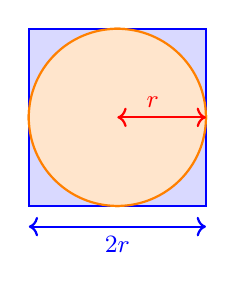
\begin{tikzpicture}[scale=0.75]
  \draw[thick, blue] (0,0) rectangle (3,3);
  \draw[thick, orange] (1.5,1.5) circle (1.5cm);
  \fill (1.5,1.5) circle (0.04);

  % Shade corners to show wasted space
  \begin{scope}
    \clip (0,0) rectangle (3,3);
    \fill[blue!15] (0,0) rectangle (3,3);
    \fill[orange!20] (1.5,1.5) circle (1.5cm);
  \end{scope}
  \draw[thick, blue] (0,0) rectangle (3,3);
  \draw[thick, orange] (1.5,1.5) circle (1.5cm);

  \draw[red, thick, <->] (1.5,1.5) -- ++(0:1.5);
  \node[red] at (2.1,1.75) {\small $r$};
  \draw[blue, thick, <->] (0,-0.35) -- (3,-0.35);
  \node[blue] at (1.5,-0.65) {\small $2r$};

\end{tikzpicture}
\end{center}

\column{0.65\textwidth}
\small
\begin{enumerate}
  \begin{multicols}{2}
    \item $5 \times 5 = \ashowq{25}$
    \item $8^2 = \ashowq{64}$
  \end{multicols}
  \begin{multicols}{2}
    \item $2.5^2 = \ashowq{6.25}$
    \item $3.14 \times 9 = \ablank{28.26}$
  \end{multicols}
  \item \ealpara{\ealkeytr{Pole} \ealkeytr{prostokąta} o wymiarach $7$ cm $\times$ $4$ cm $= \ashowq{28\,\text{cm}^2}$}{\ealkey{Area} of a $7$ cm $\times$ $4$ cm \ealkey{rectangle} $= \ashowq{28\,\text{cm}^2}$}
  \item \ealpara{Jaki \ealkeytr{ułamek} kąta $360^\circ$ stanowi $90^\circ$? \ashow{$\frac{1}{4}$}}{What \ealkey{fraction} of $360^\circ$ is $90^\circ$? \ashow{$\frac{1}{4}$}}
\end{enumerate}

\begin{enumerate}
  \setcounter{enumi}{6}
  \item \ealpara{Napisz \ealkeytr{wyrażenie} na \ealkeytr{pole} \ealkeytr{koła} na rysunku \ashow{$\pi r^2$}}{Write an \ealkey{expression} for the \ealkey{area} of the \ealkey{circle} in the picture \ashow{$\pi r^2$}}
  \item \ealpara{Napisz \ealkeytr{wyrażenie} na \ealkeytr{pole} zacieniowanego niebieskiego obszaru na rysunku \ashow{$4r^2-\pi r^2$}}{Write an \ealkey{expression} for the \ealkey{area} of the shaded blue region in the picture \ashow{$4r^2-\pi r^2$}}
  \item \ealpara{Jeśli \ealkeytr{kwadrat} ma \ealkeytr{obwód} 48cm, jakie jest \ealkeytr{pole} zacieniowanego niebieskiego obszaru? \ashow{$30.96\,\text{cm}^2$}}{If the \ealkey{square} has a \ealkey{perimeter} of 48cm, what is the \ealkey{area} of the shaded blue region? \ashow{$30.96\,\text{cm}^2$}}
\end{enumerate}

\end{columns}
\end{frame}

%------------------------------------------------
% SLIDE 4: Full Retrieval + Fluency with Area + Spot the Error
%------------------------------------------------
\begin{frame}{Starter}

\ealpara{Rozgrzewka}{Starter}

\begin{columns}

\column{0.35\textwidth}
\begin{center}
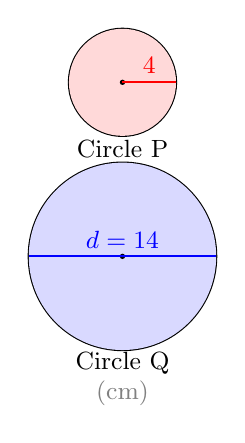
\begin{tikzpicture}[scale=0.85]

  % Two circles for comparison
  \draw[thick] (0, 2.2) circle (0.8cm);
  \fill[red!15] (0,2.2) circle (0.8cm);
  \fill (0,2.2) circle (0.04);
  \draw[red, thick] (0,2.2) -- ++(0:0.8);
  \node[red] at (0.4, 2.45) {\small $4$};
  \node at (0, 1.2) {\small Circle P};

  \draw[thick] (0,-0.4) circle (1.4cm);
  \fill[blue!15] (0,-0.4) circle (1.4cm);
  \fill (0,-0.4) circle (0.04);
  \draw[blue, thick] (-1.4,-0.4) -- (1.4,-0.4);
  \node[blue] at (0,-0.15) {\small $d=14$};
  \node at (0,-2.0) {\small Circle Q};

  \node[gray] at (0,-2.45) {\small (cm)};

\end{tikzpicture}
\end{center}

\column{0.65\textwidth}
\small
\begin{enumerate}
  \begin{multicols}{2}
    \item $9^2 = \ashowq{81}$
    \item $3.5^2 = \ashowq{12.25}$
  \end{multicols}
  \begin{multicols}{2}
    \item $3.14 \times 16$ \ashow{$=50.24$}
    \item $3.14 \times 49$ \ashow{$=153.86$}
  \end{multicols}
  \item \ealpara{Podziel na pół $14$ cm. \quad Następnie \ealkeytr{podnieś do kwadratu} swoją odpowiedź. \ashow{$7$ cm, więc $49\,\text{cm}^2$}}{Halve $14$ cm. \quad Then \ealkey{square} your answer. \ashow{$7$ cm, so $49\,\text{cm}^2$}}
  \item \ealpara{Pewien \ealkeytr{kwadrat} ma \ealkeytr{pole} $64$ cm$^2$. Jaka jest długość jego boku \ashowq{$8$ cm}}{A \ealkey{square} has \ealkey{area} $64$ cm$^2$. What is its side length \ashowq{$8$ cm}}
\end{enumerate}

\begin{enumerate}
  \setcounter{enumi}{6}
  \item \ealpara{\textbf{Znajdź błąd:} \textit{``\ealkeytr{Koło} Q ma \ealkeytr{średnicę} $14$ cm, więc jego \ealkeytr{pole} wynosi $\pi \times 14^2 \approx 615$ cm$^2$.''} Jaki błąd popełniono? Napisz poprawne rozwiązanie. \ashow{Użyto \ealkeytr{średnicy} zamiast \ealkeytr{promienia}: $\pi \times 7^2 \approx 153.86\,\text{cm}^2$.}}{\textbf{Spot the mistake:} \textit{``\ealkey{Circle} Q has \ealkey{diameter} $14$ cm, so its \ealkey{area} is $\pi \times 14^2 \approx 615$ cm$^2$.''} What error was made? Write the correct solution. \ashow{Used \ealkey{diameter} not \ealkey{radius}: $\pi \times 7^2 \approx 153.86\,\text{cm}^2$.}}
  \item \ealpara{\textbf{\ealkeytr{Koło} P}, \ealkeytr{promień} $4$ cm. Znajdź: (a) \ealkeytr{pole} \ablank{$50.24\,\text{cm}^2$} \quad (b) \ealkeytr{obwód} \ablank{25.12\,\text{cm}}.}{\textbf{\ealkey{Circle} P}, \ealkey{radius} $4$ cm. Find: (a) the \ealkey{area} \ablank{$50.24\,\text{cm}^2$} \quad (b) the \ealkey{circumference} \ablank{25.12\,\text{cm}}.}
  \item \ealpara{\textbf{\ealkeytr{Koło} Q}, \ealkeytr{średnica} $14$ cm. Znajdź: (a) \ealkeytr{pole} \ablank{$153.86\,\text{cm}^2$} \quad (b) \ealkeytr{obwód} \ablank{43.96\,\text{cm}}.}{\textbf{\ealkey{Circle} Q}, \ealkey{diameter} $14$ cm. Find: (a) the \ealkey{area} \ablank{$153.86\,\text{cm}^2$} \quad (b) the \ealkey{circumference} \ablank{43.96\,\text{cm}}.}
  \item \ealpara{Które ma większe \ealkeytr{pole}, P czy Q? O około ile cm$^2$? \ashow{Q, o około $103.62\,\text{cm}^2$.}}{Which has the greater \ealkey{area}, P or Q? By approximately how many cm$^2$? \ashow{Q, by approximately $103.62\,\text{cm}^2$.}}
\end{enumerate}

\end{columns}
\end{frame}

\end{document}